\documentclass[12pt]{article}
\setlength{\parindent}{0pt}

%%%%%%%%%%%%%%%%%%%%%%%%%%%%%%%%%%%%%%%%%%%%%%%%%%%%%%%%%%%%%%%%%%%%
% PAQUETES
%%%%%%%%%%%%%%%%%%%%%%%%%%%%%%%%%%%%%%%%%%%%%%%%%%%%%%%%%%%%%%%%%%%%
\usepackage[left=3cm, right=3cm, top=2.5cm, bottom=2.5cm]{geometry}
\usepackage{graphicx}
\usepackage{amsmath}
\usepackage{longtable}
\usepackage{subcaption}
\usepackage{booktabs}
\usepackage{enumitem}
\usepackage[hidelinks]{hyperref}
\usepackage[english]{babel}
\usepackage{csquotes}
\usepackage{tikz}
\usetikzlibrary{positioning, arrows.meta}
\usepackage{caption}
\usepackage{booktabs}
\usepackage{float}
\usepackage[
    backend=biber,
    style=apa,
    sorting=none
]{biblatex}
\addbibresource{references.bib}
\usepackage[font=footnotesize]{caption}
\usepackage{listings}
\usepackage{xcolor}

% Configure listings package
\lstset{
    basicstyle=\ttfamily\footnotesize,
    breaklines=true,
    breakatwhitespace=true,
    frame=single,
    numbers=left,
    numberstyle=\tiny\color{gray},
    keywordstyle=\color{blue},
    stringstyle=\color{red},
    commentstyle=\color{green!60!black}
}

%%%%%%%%%%%%%%%%%%%%%%%%%%%%%%%%%%%%%%%%%%%%%%%%%%%%%%%%%%%%%%%%%%%%
% INICIO DOCUMENTO
%%%%%%%%%%%%%%%%%%%%%%%%%%%%%%%%%%%%%%%%%%%%%%%%%%%%%%%%%%%%%%%%%%%%
\begin{document}
%%%%%%%%%%%%%%%%%%%%%%%%%%%%%%%%%%%%%%%%%%%%%%%%%%%%%%%%%%%%%%%%%%%%
% PORTADA
%%%%%%%%%%%%%%%%%%%%%%%%%%%%%%%%%%%%%%%%%%%%%%%%%%%%%%%%%%%%%%%%%%%%
\begin{titlepage}
    \begin{center}
        \textbf{\Huge{Design and Implementation of a 3-Tier Lakehouse for Mobility Data Analysis}}\\
        \vspace{400pt}
        Borja Albert Gramaje \& Joan Fernández Navarro
    \end{center}

    \hrule 
    \vspace{-5pt}
        \begin{center}
    	\Large{
            B\hspace{4pt}I\hspace{4pt}G\hspace{12pt}            D\hspace{4pt}A\hspace{4pt}T\hspace{4pt}A\\          E\hspace{4pt}N\hspace{4pt}G\hspace{4pt}I\hspace{4pt}N\hspace{4pt}E\hspace{4pt}E\hspace{4pt}R\hspace{4pt}I\hspace{4pt}N\hspace{4pt}G\hspace{12pt}            A\hspace{4pt}N\hspace{4pt}D\hspace{12pt}            T\hspace{4pt}E\hspace{4pt}C\hspace{4pt}H\hspace{4pt}N\hspace{4pt}O\hspace{4pt}L\hspace{4pt}O\hspace{4pt}G\hspace{4pt}I\hspace{4pt}E\hspace{4pt}S
        }\\
        \vspace{5pt}
        \normalsize{
            Master's Degree in Computational Engineering and Industrial Mathematics
        }
    \end{center}
    \vspace{-5pt}
    \hrule
    \vspace{30pt}
    \begin{figure}[h] 
		\flushright
        \includegraphics[height=0.1\linewidth]{images/upv-logo.jpg}
    \end{figure}
\end{titlepage}

\pagebreak
%%%%%%%%%%%%%%%%%%%%%%%%%%%%%%%%%%%%%%%%%%%%%%%%%%%%%%%%%%%%%%%%%%%%
% ÍNDICE
%%%%%%%%%%%%%%%%%%%%%%%%%%%%%%%%%%%%%%%%%%%%%%%%%%%%%%%%%%%%%%%%%%%%
\begin{center}
    \tableofcontents
\end{center}

\pagebreak
\addcontentsline{toc}{section}{List of Figures}
\listoffigures
\addcontentsline{toc}{section}{List of Tables}
\listoftables

\pagebreak
%%%%%%%%%%%%%%%%%%%%%%%%%%%%%%%%%%%%%%%%%%%%%%%%%%%%%%%%%%%%%%%%%%%%
% Introduction
%%%%%%%%%%%%%%%%%%%%%%%%%%%%%%%%%%%%%%%%%%%%%%%%%%%%%%%%%%%%%%%%%%%%
\section{Introduction}

The objective of this project is the design and implementation of a robust, three-tier Data Lakehouse architecture specifically engineered to analyze large-scale mobility patterns across Spain. The core of this infrastructure is built upon DuckLake, leveraging PostgreSQL for metadata cataloging and schema versioning, alongside an S3-compatible object storage layer. For this implementation, RustFS is utilized to emulate S3 behavior locally, providing high-performance storage for data files in Parquet and CSV formats while maintaining cloud-native compatibility.

The system is structured into three distinct refinement layers to ensure data integrity and analytical readiness:
\begin{itemize}
    \item \textbf{Bronze Layer (Raw):} This staging area serves as the entry point for raw datasets ingested directly from public sources. It preserves the original state of the information for auditability.
    \item \textbf{Silver Layer (Core):} In this intermediate tier, data undergoes rigorous cleaning, standardization, and integration. Here, the system performs complex joins between mobility data and socioeconomic indicators, handles anomalies, and normalizes units.
    \item \textbf{Gold Layer (Mart):} The final layer consists of business-ready data products and pre-computed analytical models. This tier stores the aggregated results and high-level insights.
\end{itemize}

The data processed within this Lakehouse is sourced from two primary Spanish public institutions: the Ministry of Transport, Mobility and Urban Agenda (MITMA) and the National Statistics Institute (INE). The MITMA provides high-frequency mobility flows and origin-destination matrices, using 2023 as a baseline year for structural analysis. This is complemented by INE datasets, which contribute critical demographic profiles (population density, age, and gender) and economic indicators (income levels and business activity) to provide context to the movement patterns.

To demonstrate the practical applicability of this infrastructure for urban planning and territorial management, the system is evaluated through three specific Business Questions. These questions focus on characterizing typical travel rhythms, identifying underserved corridors, and classifying the functional use of urban zones, all of which are detailed in the following section.

%%%%%%%%%%%%%%%%%%%%%%%%%%%%%%%%%%%%%%%%%%%%%%%%%%%%%%%%%%%%%%%%%%%%
% Introduction
%%%%%%%%%%%%%%%%%%%%%%%%%%%%%%%%%%%%%%%%%%%%%%%%%%%%%%%%%%%%%%%%%%%%
\section{Business and analytical objectives}

\subsection{Business Question 1: Typical mobility day}
The primary objective of this analysis is to establish a comprehensive baseline of regional movement by characterizing the structural rhythms of a ``typical'' day within a specific region and a given date range. By aggregating hourly origin-destination flows, the goal is to move beyond raw data to understand the underlying temporal patterns of demand. This involves identifying and distinguishing between different mobility signatures, such as the concentrated commuting flows between municipalities or which are the peek hours in a specific municipality.

From an analytical perspective, the maps and plots created serve as the foundation for operational efficiency. For example, by analyzing the average hourly cars flow, a transport planner can determine if the peak 8:00 AM rush hour is the correct time to start sending packages to the city or is better to wait until 9:00 AM. This typical day profile allows for data-driven decisions on where and when to allocate transit resources most effectively.

\subsection{Business Question 2: Infrastructure gaps}
This objective is designed to identify where transport infrastructure is most lacking by highlighting discrepancies between potential and actual mobility. The analysis employs a theoretical``Gravity Model'' to estimate potential demand based on the socioeconomic mass of various zones, specifically their population and business activity, and the distance between them. By comparing these theoretical estimates against the real-world trip volumes recorded in the mobility matrices, the analysis produces ``mismatch ratio''.

The analytical value of this comparison lies in the identification of underserved corridors. For instance, if the model predicts a high volume of trips between a densely populated residential municipality and a nearby non-residential region, but the actual data shows very few trips, it reveals a significant infrastructure gap. This insight is critical for prioritizing public investment, as it points to specific areas where a new transport method would satisfy a large latent demand that is currently being suppressed by poor infrastructure.

\subsection{Business Question 3: Functional type clustering}
The goal of this objective is to characterize the functional role of different geographic zones based on their specific mobility behaviours rather than administrative labels. By clustering zones according to their inbound and outbound trip patterns throughout the day, we can distinguish between areas that serve as residential hubs and those that act as centers of activity.

A clear example of the real-world applicability of this question is the characterization of the Valencia Metropolitan Area. By selecting this specific polygon, the analysis can identify which municipalities function as ``dormitory towns'', those that see a massive outbound flow of residents in the morning, and locate the primary employment hubs where those trips are concentrated. Understanding how the population redistributes itself based on daily commutes allows for more effective territorial planning, such as developing local services in dormitory towns to reduce the need for long-distance travel or improving high-capacity access to identified work focuses.


%%%%%%%%%%%%%%%%%%%%%%%%%%%%%%%%%%%%%%%%%%%%%%%%%%%%%%%%%%%%%%%%%%%%
% Methodology
%%%%%%%%%%%%%%%%%%%%%%%%%%%%%%%%%%%%%%%%%%%%%%%%%%%%%%%%%%%%%%%%%%%%
\section{Methodology}

\subsection{Data sources}

The Lakehouse architecture ingests data from three primary sources, each requiring different extraction mechanisms and handling strategies. Table~\ref{tab:data_sources_summary} provides an overview of the data sources, their formats, and update frequencies.

\begin{table}[H]
\centering
\begin{tabular}{p{3cm} p{4cm} p{2.5cm} p{3.5cm}}
\toprule
\textbf{Source} & \textbf{Data Type} & \textbf{Format} & \textbf{Frequency} \\
\midrule
MITMA & Mobility matrices, Zoning & CSV.GZ, Shapefiles & Daily \\
INE & Socioeconomic indicators & JSON (REST API) & Annual \\
OpenHolidays & National holidays & JSON (REST API) & On-demand \\
\bottomrule
\end{tabular}
\caption{Summary of data sources and their characteristics}
\label{tab:data_sources_summary}
\end{table}

\subsubsection*{MITMA (Ministry of Transport, Mobility and Urban Agenda)}

The MITMA provides mobility data through an RSS feed that publishes daily updates of origin-destination matrices. The data extraction process involves parsing the RSS XML feed to identify available CSV files, filtering by date range and zone type, and downloading compressed files for processing.

\textbf{RSS Feed and URL Structure:}

The primary data source is the MITMA RSS feed located at \url{https://movilidad-opendata.mitma.es/RSS.xml}. This feed contains links to daily CSV files organized by zone type (\texttt{municipios}, \texttt{distritos}, or \texttt{gau}) and dataset type. The system parses this XML feed using regular expressions to extract URLs matching the following pattern:

\begin{lstlisting}[language=bash]
https://movilidad-opendata.mitma.es/estudios_basicos/
  por-{zone_type}/viajes/ficheros-diarios/
  {YYYY-MM}/{YYYYMMDD}_Viajes_{zone_type}.csv.gz
\end{lstlisting}

For example, a file for March 6, 2023 at the municipality level would be:
\begin{lstlisting}[language=bash]
https://movilidad-opendata.mitma.es/estudios_basicos/
  por-municipios/viajes/ficheros-diarios/2023-03/
  20230306_Viajes_municipios.csv.gz
\end{lstlisting}

\textbf{Origin-Destination Data Structure:}

Each CSV file contains origin-destination mobility matrices with the structure shown in Table~\ref{tab:mitma_od_structure}. Files are compressed using gzip, with typical sizes ranging from 50-100 MB per day for municipality-level data.

\begin{table}[H]
\centering
\begin{tabular}{p{2.5cm} p{3cm} p{6cm}}
\toprule
\textbf{Column} & \textbf{Type (Bronze)} & \textbf{Description} \\
\midrule
\texttt{fecha} & TIMESTAMP & Date parsed from YYYYMMDD format \\
\texttt{periodo} & VARCHAR & Hour of day (0-23) \\
\texttt{origen} & VARCHAR & Origin zone identifier \\
\texttt{destino} & VARCHAR & Destination zone identifier \\
\texttt{viajes} & VARCHAR & Number of trips (as string) \\
\texttt{viajes\_km} & VARCHAR & Total distance traveled (as string) \\
\texttt{distancia} & VARCHAR & Distance category or band \\
\texttt{residencia} & VARCHAR & Residence classification \\
\bottomrule
\end{tabular}
\caption{Structure of MITMA origin-destination CSV files}
\label{tab:mitma_od_structure}
\end{table}

The extraction process downloads files sequentially to avoid overwhelming local resources, then stages them in RustFS for parallel processing by Cloud Run Jobs.

\textbf{Zonification Data:}

In addition to mobility matrices, MITMA provides zoning reference data including geometric boundaries (polygons) for each zone. This data is extracted from the RSS feed by matching patterns for Shapefile components (\texttt{.shp}, \texttt{.shx}, \texttt{.dbf}, \texttt{.prj}) and supplementary CSV files containing zone names and population metadata. The geometry data is stored as Well-Known Text (WKT) strings in the Bronze layer.

\textbf{MITMA-INE Relations:}

A critical mapping table is extracted from a static CSV file published by MITMA at \url{https://movilidad-opendata.mitma.es/zonificacion/relacion_ine_zonificacionMitma.csv}. This table establishes the correspondence between MITMA zone identifiers and INE municipality codes, enabling integration of mobility data with socioeconomic indicators. The file uses pipe-delimited format (\texttt{|}) and is read directly from its URL using DuckDB's \texttt{read\_csv()} function.

\subsubsection*{INE (National Statistics Institute)}

The INE provides socioeconomic and demographic data through a REST API that returns JSON responses. Unlike MITMA's file-based approach, INE data requires HTTP requests to specific endpoints with query parameters.

\textbf{API Endpoints:}

All INE data is accessed through the base URL \url{https://servicios.ine.es/wstempus/js/ES/}, with specific endpoints for different datasets as shown in Table~\ref{tab:ine_endpoints}.

\begin{table}[H]
\centering
\begin{tabular}{p{3cm} p{5cm} p{4.5cm}}
\toprule
\textbf{Dataset} & \textbf{Endpoint Pattern} & \textbf{Description} \\
\midrule
Municipalities & \texttt{VALORES\_VARIABLE/19} & Catalog of all Spanish municipalities with INE codes and names \\
Companies & \texttt{DATOS\_TABLA/3955?tip=AM\&date=\{year\}0101} & Number of registered companies per municipality and year \\
Population & \texttt{DATOS\_TABLA/29005?date=\{year\}0101:\{year\}1231} & Population counts by municipality, sex, and year \\
Income & \texttt{DATOS\_TABLA/\{id\}?date=\{year\}0101} & Average income per capita (52 table IDs: 30656-31295) \\
\bottomrule
\end{tabular}
\caption{INE API endpoints and their purposes}
\label{tab:ine_endpoints}
\end{table}

\textbf{JSON Structure and Parsing:}

INE API responses use a nested JSON structure where each municipality entry contains a \texttt{Data} array with time-series values. The population endpoint, for example, returns data in the following format:

\begin{lstlisting}[language=json]
[
  {
    "COD": "28079",
    "Nombre": "Madrid",
    "Data": [
      {"Fecha": "20230101", "Valor": 3300000},
      {"Fecha": "20220101", "Valor": 3250000}
    ]
  }
]
\end{lstlisting}

The extraction process uses DuckDB's \texttt{read\_json()} function with \texttt{format='array'} to parse these responses directly from URLs. For datasets with nested \texttt{Data} arrays, the system uses \texttt{UNNEST()} operations in the Silver layer to explode time-series data into individual rows.

\textbf{Dynamic URL Generation:}

The system generates URLs dynamically based on the target year. For income data, which spans 52 different table IDs, the system creates a list of URLs using dynamic task mapping in Airflow, enabling parallel processing of all endpoints. Each URL includes the year parameter in the format \texttt{?date=\{year\}0101} to retrieve data for the specified year.

\subsubsection*{Spanish National Holidays}

Holiday data is generated programmatically using the OpenHolidays API, which provides a standardized source of public holidays for Spain. The extraction process queries the API endpoint with the following structure:

\begin{lstlisting}[language=bash]
https://openholidaysapi.org/PublicHolidays?
  countryIsoCode=ES&
  languageIsoCode=ES&
  validFrom={year}-01-01&
  validTo={year}-12-31
\end{lstlisting}

The API returns a JSON array of holiday objects, from which the system extracts only nationwide holidays (\texttt{nationwide = true}), filtering out regional holidays. Each record contains:
\begin{itemize}
    \item \texttt{startDate}: Holiday date (parsed to DATE type)
    \item \texttt{name[1].text}: Holiday name in Spanish
\end{itemize}

This data is used in the Silver layer to enrich mobility records with \texttt{is\_holiday} flags, enabling temporal analysis that distinguishes between regular days and national holidays.

\subsubsection*{Extraction Workflow}

The data extraction process follows a consistent five-phase pattern across all sources, ensuring reliability and idempotency:

\begin{enumerate}
    \item \textbf{URL Discovery:} 
    \begin{itemize}
        \item MITMA: Parse RSS feed using regular expressions to extract file URLs
        \item INE: Generate URLs based on year and table IDs programmatically
        \item Holidays: Construct API URL with year parameters
    \end{itemize}
    
    \item \textbf{Idempotency Check:} Filter URLs against existing \texttt{source\_file} or \texttt{source\_url} columns in Bronze tables to skip already-ingested data. This enables safe re-execution of DAGs without data duplication.
    
    \item \textbf{Download/Request:} 
    \begin{itemize}
        \item MITMA: Download CSV files sequentially to local staging (RustFS bucket)
        \item INE and Holidays: Execute HTTP requests directly from Cloud Run Jobs
    \end{itemize}
    
    \item \textbf{Ingestion:} Use DuckDB's native functions (\texttt{read\_csv()}, \texttt{read\_json()}) to load data into Bronze tables with metadata tracking (\texttt{loaded\_at}, \texttt{source\_file}/\texttt{source\_url}).
    
    \item \textbf{Cleanup:} Remove temporary staging files from RustFS after successful ingestion to manage storage costs.
\end{enumerate}

This approach ensures reliable, idempotent data ingestion while maintaining full lineage tracking through source URL/file columns in the Bronze layer, enabling complete auditability and reprocessing capabilities.

\subsection{Technical environment and infrastructure}

Given the large volume of mobility data processed in this project (hundreds of millions of records across multiple years), a cloud-based infrastructure was essential to handle the computational requirements. The system architecture leverages Apache Airflow for orchestration, DuckDB (via DuckLake) as the analytical engine, and Google Cloud Platform services for scalable compute resources.

\subsubsection*{Apache Airflow}
Apache Airflow 3.x serves as the workflow orchestration platform, managing the entire data pipeline through Directed Acyclic Graphs (DAGs). The system implements a dataset-driven architecture where Bronze layer DAGs publish completion signals that trigger downstream Silver layer transformations. This ensures data dependencies are respected and enables automatic pipeline execution when source data becomes available. Airflow manages task scheduling, retries, dynamic task mapping for parallel processing, and provides comprehensive monitoring and logging capabilities.

\subsubsection*{DuckDB and DuckLake}
DuckDB, accessed through the DuckLake interface, functions as the analytical database engine. DuckLake extends DuckDB by providing S3-compatible object storage integration and PostgreSQL-based metadata cataloging. This architecture allows for:
\begin{itemize}
    \item \textbf{Schema-on-read flexibility:} Bronze layer tables use flexible schemas with all columns as \texttt{VARCHAR} to accommodate varying source formats
    \item \textbf{Partitioning:} Tables are partitioned by temporal dimensions (year, month, day) to optimize query performance
    \item \textbf{Spatial operations:} The spatial extension enables geometric calculations for zone centroids and distance computations
    \item \textbf{Metadata management:} PostgreSQL stores table schemas, enabling versioning and schema evolution tracking
\end{itemize}

\subsubsection*{Google Cloud Platform}
Due to the computational intensity of processing mobility matrices (which can exceed 250,000 origin-destination pairs per day), local resources were insufficient. Google Cloud Platform provides the necessary scalability:

\begin{itemize}
    \item \textbf{Cloud Run Jobs:} Heavy computational tasks execute in Cloud Run Jobs with dedicated resources (32GB RAM, 8 CPUs). This includes:
    \begin{itemize}
        \item Bulk data ingestion from MITMA RSS feeds (via intermediate staging)
        \item Complex SQL transformations requiring large memory allocations
        \item Distance calculations across all zone pairs (cross-joins of thousands of zones)
        \item Gravity model calibration and mismatch computations
    \end{itemize}
    \item \textbf{Cloud Build:} Automated container builds and deployments for the Cloud Run Job images, ensuring consistent execution environments
    \item \textbf{Object Storage Integration:} RustFS (S3-compatible) serves as the local object storage layer, while maintaining compatibility with cloud-native S3 APIs for future migration
\end{itemize}

\textbf{Cross-cloud connectivity challenges:}

A significant technical challenge encountered during implementation was the inability to directly access MITMA's AWS-hosted S3 bucket from Google Cloud Run Jobs. Attempts to use DuckDB's \texttt{read\_csv()} function with HTTP URLs from Cloud Run consistently resulted in HTTP 500 errors, a problem documented in various forums for similar cross-cloud scenarios involving other government data sources. This limitation necessitated the implementation of a hybrid architecture where initial data downloads occur locally (avoiding cross-cloud issues) before staging files in RustFS for Cloud Run processing.

The hybrid architecture balances cost efficiency (local processing for lightweight tasks) with scalability (cloud execution for compute-intensive operations). Airflow workers execute simple tasks locally, while delegating heavy workloads to Cloud Run Jobs that scale automatically based on demand. This approach, while not ideal, provides a functional solution that works around cloud provider interoperability limitations.

\subsection{Lakehouse architecture}

The three-tier Medallion architecture (Bronze, Silver, Gold) ensures data quality progression from raw ingestion to business-ready analytics. Each layer applies increasingly sophisticated transformations while maintaining data lineage and auditability. The architecture implements schema-on-read in Bronze, schema-on-write in Silver, and optimized analytical schemas in Gold.

\subsubsection{Bronze Layer}

The Bronze Layer serves as the immutable landing zone for all raw data sources. This layer preserves the original state of ingested data without business logic transformations, ensuring full auditability and enabling reprocessing if source schemas change. All tables implement a flexible schema where columns are stored as \texttt{VARCHAR} to accommodate varying source formats and prevent type-related ingestion failures.

\subsubsection*{Design principles}
\begin{itemize}
    \item \textbf{Schema flexibility:} All columns stored as \texttt{VARCHAR} to handle inconsistent source formats
    \item \textbf{Metadata tracking:} Every record includes \texttt{loaded\_at} (timestamp) and \texttt{source\_file} or \texttt{source\_url} for lineage tracking
    \item \textbf{Idempotency:} Duplicate detection based on \texttt{source\_file}/\texttt{source\_url} prevents reprocessing of already-ingested data
    \item \textbf{Partitioning:} Temporal partitioning by date enables efficient incremental processing
    \item \textbf{No data loss:} All original columns preserved, even if not used in downstream layers
\end{itemize}

\subsubsection*{Data sources and tables}

The Bronze layer ingests data from three primary sources:

\textbf{MITMA (Ministry of Transport, Mobility and Urban Agenda):}
\begin{itemize}
    \item \texttt{bronze\_mitma\_od\_municipios}: Origin-destination mobility matrices by municipality, date, and hour. Data extracted from MITMA RSS feeds, with each CSV file containing daily trip volumes between zone pairs.
    \item \texttt{bronze\_mitma\_municipios}: Zoning reference data including geometric boundaries (polygons) for each municipality.
    \item \texttt{bronze\_mitma\_ine\_relations}: Mapping table connecting MITMA zone identifiers to INE municipality codes.
\end{itemize}

\textbf{INE (National Statistics Institute):}
\begin{itemize}
    \item \texttt{bronze\_ine\_municipios}: Catalog of Spanish municipalities with INE codes and names.
    \item \texttt{bronze\_ine\_empresas\_municipio}: Number of registered companies per municipality and year (JSON API format).
    \item \texttt{bronze\_ine\_poblacion\_municipio}: Population counts by municipality, sex, and year.
    \item \texttt{bronze\_ine\_renta\_municipio}: Average income per capita by municipality and year.
\end{itemize}

Significant development effort was invested in implementing dynamic data retrieval from the INE REST API, enabling automated HTTP requests that eliminate the need for manual data imports. This approach provides real-time access to socioeconomic indicators and ensures data freshness without requiring manual intervention or file downloads. The API integration handles JSON responses with nested data structures, requiring careful parsing and normalization to extract year-specific values from the \texttt{Data} arrays.

\textbf{Derived data:}
\begin{itemize}
    \item \texttt{bronze\_spanish\_holidays}: National holidays generated programmatically using Python's \texttt{holidays} library, used to enrich mobility data with temporal flags.
\end{itemize}

\subsubsection*{Ingestion workflow}

The Bronze layer implements a three-phase ingestion process for large datasets (particularly MITMA OD data). However, this workflow was necessitated by a critical infrastructure compatibility issue encountered during development:

\textbf{Cloud-to-cloud connectivity issue:}

During initial implementation, attempts to read MITMA CSV files directly from their S3 bucket (hosted on AWS infrastructure) using DuckDB's \texttt{read\_csv()} function from Google Cloud Run Jobs consistently resulted in HTTP 500 errors. This issue, documented in various forums for similar cross-cloud scenarios, appears to stem from network routing or authentication challenges when accessing AWS-hosted S3 buckets from Google Cloud infrastructure. After extensive experimentation and multiple cloud deployment iterations, a functional workaround was implemented.

\textbf{Three-phase workaround implementation:}

\begin{enumerate}
    \item \textbf{Download phase:} Airflow workers running locally download CSV files from MITMA RSS feeds via HTTP. This local download avoids the cross-cloud connectivity issues.
    \item \textbf{Upload phase:} Downloaded files are uploaded to a separate RustFS bucket (distinct from the main data lake bucket) to serve as temporary staging storage. This intermediate step ensures files are accessible to Cloud Run Jobs without requiring direct access to the MITMA S3 bucket.
    \item \textbf{Processing phase:} Cloud Run Jobs execute in parallel, reading from the RustFS staging bucket and performing MERGE operations into DuckDB tables. This phase handles the computationally intensive parsing and type inference.
    \item \textbf{Cleanup phase:} Temporary files are removed from the RustFS staging bucket after successful ingestion to manage storage costs and maintain separation between staging and production data.
\end{enumerate}

While this approach is not the most elegant solution, it provides a functional workaround that enables reliable data ingestion. The architecture enables parallel processing of multiple files while offloading heavy computation to cloud resources. The workflow uses dynamic task mapping in Airflow to process batches of URLs concurrently, with each batch containing 10 files by default (configurable via DAG parameters). Future improvements could explore alternative approaches such as using Google Cloud Storage as an intermediate staging area or implementing proxy services to handle cross-cloud connectivity.

\subsubsection*{Tracking and idempotency}

To ensure idempotent execution, the Bronze layer tracks ingested files using the \texttt{source\_file} column (for CSV sources) or \texttt{source\_url} (for JSON API sources). Before processing, URLs are filtered against existing records to skip already-ingested files. This allows:
\begin{itemize}
    \item Safe re-execution of DAGs without data duplication
    \item Incremental processing of new data only
    \item Recovery from partial failures by resuming from the last successfully processed file
\end{itemize}

\subsubsection{Silver Layer}

The Silver Layer applies rigorous data quality transformations, type casting, and integration logic to produce clean, standardized datasets ready for analytical consumption. This layer implements schema-on-write, enforcing correct data types and business rules while maintaining referential integrity across related tables.

\subsubsection*{Design principles}
\begin{itemize}
    \item \textbf{Type safety:} All columns cast to appropriate types (\texttt{TIMESTAMP}, \texttt{DOUBLE}, \texttt{BOOLEAN}, etc.)
    \item \textbf{Data quality:} Null filtering, outlier detection, and validation rules applied consistently
    \item \textbf{Deduplication:} \texttt{DISTINCT} operations and \texttt{MERGE INTO} statements prevent duplicate records
    \item \textbf{Enrichment:} Calculated fields added (e.g., \texttt{is\_weekend}, \texttt{is\_holiday}, \texttt{viajes\_per\_capita})
    \item \textbf{Spatial processing:} Geometric operations for zone boundaries and centroid calculations
    \item \textbf{Integration:} JOINs between MITMA and INE data sources using normalized mapping tables
\end{itemize}

\subsubsection*{Core transformation tables}

\textbf{\texttt{silver\_mitma\_ine\_mapping}:} This foundational table establishes the relationship between MITMA zone identifiers and INE municipality codes. The transformation applies name normalization (accent removal, lowercase conversion, whitespace trimming) to enable fuzzy matching between source systems. The table serves as the join key for integrating mobility data with socioeconomic indicators.

\textbf{\texttt{silver\_zones}:} Reference table containing spatial zone definitions with geometric properties. Transformations include:
\begin{itemize}
    \item Geometry conversion: \texttt{ST\_GeomFromText()} parses WKT strings, \texttt{ST\_Multi()} ensures multi-polygon compatibility
    \item Centroid calculation: \texttt{ST\_Centroid()} computes geometric centers for distance calculations
    \item Coverage filtering: Only zones with valid MITMA-INE mappings are included
\end{itemize}

\textbf{\texttt{silver\_mitma\_od}:} Cleaned origin-destination mobility flows. Key transformations:
\begin{itemize}
    \item Temporal parsing: Combines date and hour fields using \texttt{strptime(fecha || LPAD(periodo), '\%.Y\%m\%d\%H')} to create proper \texttt{TIMESTAMP} values
    \item Type casting: \texttt{viajes} and \texttt{viajes\_km} converted to \texttt{DOUBLE}
    \item Enrichment: \texttt{is\_weekend} and \texttt{is\_holiday} flags derived from date calculations and holiday table lookups
    \item Filtering: Excludes records where \texttt{origen = 'externo'} (external zones not in the zone catalog)
    \item Aggregation: Sums trip volumes when multiple demographic segments exist for the same origin-destination-date combination
    \item Partitioning: Table partitioned by \texttt{year(fecha), month(fecha), day(fecha)} for query optimization
\end{itemize}

\textbf{\texttt{silver\_mitma\_distances}:} Precomputed Euclidean distances between all zone pairs. The calculation uses spherical distance (\texttt{ST\_Distance\_Sphere()}) between zone centroids, divided by 1000 to convert meters to kilometers. The cross-join is filtered to unique pairs (\texttt{WHERE o.id < d.id}) to avoid duplicate distance calculations.

\textbf{\texttt{silver\_ine\_all}:} Consolidated table joining all INE socioeconomic indicators with zone identifiers. This table performs LEFT JOINs from \texttt{silver\_zones} to individual INE tables (empresas, poblacion, renta), using \texttt{COALESCE()} to handle missing data with default values of 0. The table includes a \texttt{year} column extracted from processing parameters to support multi-year analyses.


\subsubsection*{Data quality metrics}

The \texttt{silver\_mitma\_od\_quality} table provides diagnostic metrics for data quality assessment:
\begin{itemize}
    \item \textbf{Normalized metrics:} \texttt{viajes\_per\_capita} and \texttt{km\_per\_capita} normalize trip volumes by origin population
    \item \textbf{Validation flags:} \texttt{flag\_negative\_viajes} and \texttt{flag\_negative\_viajes\_km} identify data quality issues
    \item \textbf{Outlier detection:} Z-score standardization (\texttt{z\_viajes\_per\_capita}) and threshold-based flagging (\texttt{flag\_outlier\_viajes\_per\_capita}) identify statistical anomalies
\end{itemize}

These metrics enable downstream filtering and provide transparency into data quality issues that may affect analytical results.

\subsubsection*{Processing workflow}

The Silver layer implements incremental batch processing to handle large date ranges efficiently. The workflow uses \texttt{SELECT DISTINCT} queries to identify unprocessed dates, avoiding the need for separate tracking tables:

\begin{enumerate}
    \item \textbf{Date identification:} A \texttt{SELECT DISTINCT} query extracts unique dates from the source table (\texttt{bronze\_mitma\_od\_municipios}), optionally filtered by DAG parameters (\texttt{start\_date}, \texttt{end\_date})
    \item \textbf{Gap detection:} The query uses \texttt{EXCEPT} to compare source dates against dates already present in the target table (\texttt{silver\_mitma\_od}), identifying only unprocessed dates
    \item \textbf{Batch creation:} Unprocessed dates are grouped into configurable batches (default: 7 days) to balance parallelism and resource usage
    \item \textbf{Parallel execution:} Batches are processed concurrently using Airflow's dynamic task mapping, with each batch executing in a Cloud Run Job for heavy computations
    \item \textbf{Idempotency:} Since only unprocessed dates are selected, re-execution of the DAG automatically skips already-processed dates without requiring explicit tracking tables
\end{enumerate}

This approach enables efficient reprocessing of specific date ranges and recovery from partial failures without reprocessing entire datasets. The same pattern is applied in the Gold layer, where \texttt{gold\_typical\_day\_od\_hourly} identifies unprocessed dates by comparing \texttt{silver\_mitma\_od} dates against existing gold table records.

\subsubsection*{Decision rationale}

Several design decisions were made during Silver layer development:

\begin{itemize}
    \item \textbf{Euclidean distance:} While road network distances would be more accurate, Euclidean distance between centroids provides sufficient approximation for the gravity model while being computationally tractable. The spherical distance calculation accounts for Earth's curvature.
    \item \textbf{Null handling:} Missing INE data is replaced with 0 rather than NULL to ensure mathematical operations (e.g., gravity model calculations) proceed without null propagation issues.
    \item \textbf{Column selection:} Some Bronze columns (e.g., demographic segmentation fields in OD data) are aggregated away in Silver to reduce table size while preserving analytical value through the aggregated \texttt{viajes} metric.
    \item \textbf{Partitioning strategy:} Temporal partitioning by date components (year, month, day) rather than a single date column enables DuckDB's query optimizer to prune partitions more effectively for date range queries.
\end{itemize}

\subsubsection*{Known technical limitations and workarounds}

During development, a critical issue was encountered with DuckLake's handling of partitioned tables when using \texttt{MERGE INTO} statements. This issue, documented in GitHub issue \#503\footnote{\url{https://github.com/duckdb/ducklake/issues/503}}, occurs when tables are partitioned using date functions (\texttt{year()}, \texttt{month()}, \texttt{day()}) and \texttt{MERGE INTO} operations attempt to update existing records. The error manifests as a type mismatch where DuckLake incorrectly attempts to apply partition functions to non-date columns during the merge operation.

Testing has confirmed that this issue is resolved in DuckLake nightly builds when using Python 3.11 and DuckDB 1.4.X, but as of the project implementation, this fix had not been released in a stable version. As a result, a workaround was implemented across all affected layers:

\textbf{Workaround implementation:}

Instead of using \texttt{MERGE INTO} with partitioned tables, the system implements an incremental processing pattern using \texttt{SELECT DISTINCT} queries to identify unprocessed dates:

\begin{enumerate}
    \item \textbf{Date identification:} A \texttt{SELECT DISTINCT} query extracts unique dates from source tables, filtered by DAG parameters (\texttt{start\_date}, \texttt{end\_date}) when provided
    \item \textbf{Gap detection:} The query compares source dates against target table dates using \texttt{EXCEPT} or \texttt{NOT IN} clauses to identify missing dates
    \item \textbf{Batch processing:} Unprocessed dates are grouped into configurable batches for parallel execution
    \item \textbf{Insert-only operations:} \texttt{INSERT INTO} statements replace \texttt{MERGE INTO}, with idempotency guaranteed by the date filtering logic
\end{enumerate}

This pattern is consistently applied across:

\begin{itemize}
    \item \textbf{Silver Layer:} \texttt{silver\_mitma\_od} and \texttt{silver\_mitma\_od\_quality} tables use \texttt{INSERT INTO} with date-based filtering to ensure only unprocessed dates are inserted
    \item \textbf{Gold Layer:} \texttt{gold\_typical\_day\_od\_hourly} implements the same pattern, comparing dates from \texttt{silver\_mitma\_od} against existing records in the gold table
    \item \textbf{Bronze Layer:} While Bronze tables use \texttt{MERGE INTO}, they are partitioned by date identity rather than date functions, avoiding the issue entirely
\end{itemize}

The workaround maintains full idempotency and enables incremental processing while avoiding the DuckLake bug. Once the fix is available in a stable release, the codebase can be migrated to use \texttt{MERGE INTO} for improved efficiency and atomicity guarantees.

\subsubsection*{Workflow diagrams}

The following diagrams illustrate the Airflow DAG structures for Bronze and Silver layer processing:

\begin{figure}[H]
    \centering
    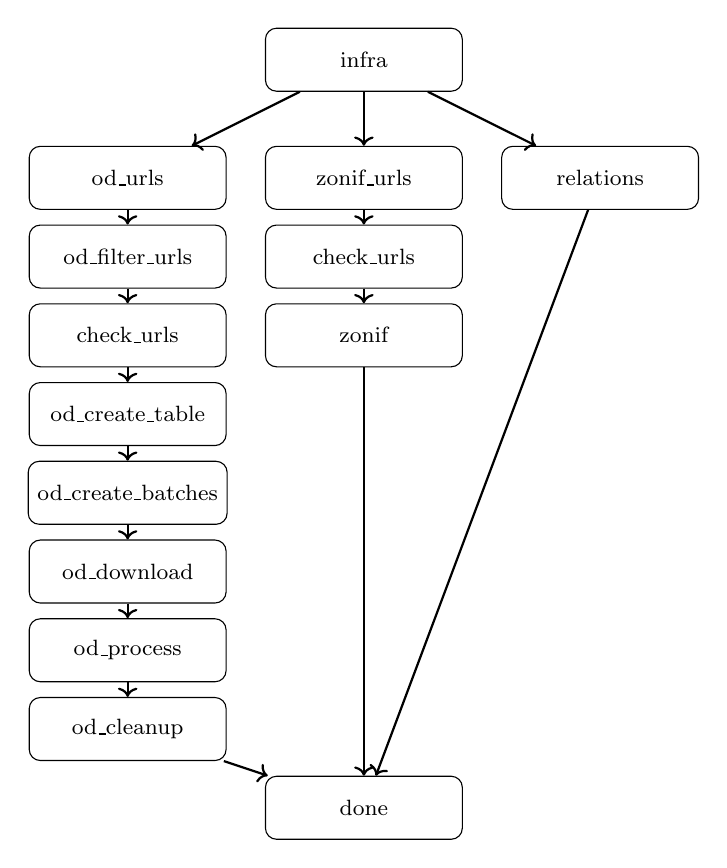
\begin{tikzpicture}[
        task/.style={
            rectangle,
            draw,
            rounded corners,
            minimum width=2.5cm,
            minimum height=0.8cm,
            align=center,
            font=\footnotesize
        },
        arrow/.style={
            ->,
            thick
        }
    ]
    
    % Bronze MITMA DAG
    \node[task] (infra) at (0, 6) {infra};
    \node[task] (od_urls) at (-3, 4.5) {od\_urls};
    \node[task] (od_filter) at (-3, 3.5) {od\_filter\_urls};
    \node[task] (od_check) at (-3, 2.5) {check\_urls};
    \node[task] (od_create) at (-3, 1.5) {od\_create\_table};
    \node[task] (od_batches) at (-3, 0.5) {od\_create\_batches};
    \node[task] (od_download) at (-3, -0.5) {od\_download};
    \node[task] (od_process) at (-3, -1.5) {od\_process};
    \node[task] (od_cleanup) at (-3, -2.5) {od\_cleanup};
    
    \node[task] (zonif_urls) at (0, 4.5) {zonif\_urls};
    \node[task] (zonif_check) at (0, 3.5) {check\_urls};
    \node[task] (zonif) at (0, 2.5) {zonif};
    
    \node[task] (ine_relations) at (3, 4.5) {relations};
    
    \node[task] (done) at (0, -3.5) {done};
    
    % Arrows
    \draw[arrow] (infra) -- (od_urls);
    \draw[arrow] (infra) -- (zonif_urls);
    \draw[arrow] (infra) -- (ine_relations);
    
    \draw[arrow] (od_urls) -- (od_filter);
    \draw[arrow] (od_filter) -- (od_check);
    \draw[arrow] (od_check) -- (od_create);
    \draw[arrow] (od_create) -- (od_batches);
    \draw[arrow] (od_batches) -- (od_download);
    \draw[arrow] (od_download) -- (od_process);
    \draw[arrow] (od_process) -- (od_cleanup);
    
    \draw[arrow] (zonif_urls) -- (zonif_check);
    \draw[arrow] (zonif_check) -- (zonif);
    
    \draw[arrow] (od_cleanup) -- (done);
    \draw[arrow] (zonif) -- (done);
    \draw[arrow] (ine_relations) -- (done);
    
    \end{tikzpicture}
    \caption{Bronze MITMA DAG workflow showing parallel task groups for OD, Zonification, and INE Relations processing.}
    \label{fig:bronze_mitma_dag}
\end{figure}

\begin{figure}[H]
    \centering
    \begin{tikzpicture}[
        task/.style={
            rectangle,
            draw,
            rounded corners,
            minimum width=2.2cm,
            minimum height=0.7cm,
            align=center,
            font=\tiny
        },
        arrow/.style={
            ->,
            thick
        },
        dataset/.style={
            ellipse,
            draw,
            minimum width=1.8cm,
            minimum height=0.6cm,
            align=center,
            font=\tiny
        }
    ]
    
    % Silver DAG
    \node[dataset] (bronze_mitma) at (-3, 6) {bronze://mitma};
    \node[dataset] (bronze_ine) at (-1, 6) {bronze://ine};
    \node[dataset] (bronze_holidays) at (1, 6) {bronze://holidays};
    
    \node[task] (start) at (-1, 4.5) {start};
    \node[task] (mapping) at (-1, 3.5) {mapping};
    \node[task] (zonif) at (-1, 2.5) {zonification};
    \node[task] (distances) at (-1, 1.5) {distances};
    
    \node[task] (od_create) at (-3.5, 3.5) {od\_create};
    \node[task] (od_batches) at (-3.5, 2.5) {od\_batches};
    \node[task] (od_check) at (-3.5, 1.5) {od\_check};
    \node[task] (od_process) at (-3.5, 0.5) {od\_process};
    
    
    \node[task] (ine_coverage) at (3.5, 3.5) {ine\_coverage};
    \node[task] (ine_all) at (3.5, 2.5) {ine\_all};
    
    \node[task] (od_quality_create) at (-1, 0) {quality\_create};
    \node[task] (od_quality_batches) at (-1, -1) {quality\_batches};
    \node[task] (od_quality_process) at (-1, -2) {quality\_process};
    
    \node[task] (done) at (-1, -3) {done};
    
    % Arrows
    \draw[arrow] (bronze_mitma) -- (start);
    \draw[arrow] (bronze_ine) -- (start);
    \draw[arrow] (bronze_holidays) -- (start);
    
    \draw[arrow] (start) -- (mapping);
    \draw[arrow] (start) -- (od_create);
    
    \draw[arrow] (mapping) -- (zonif);
    \draw[arrow] (mapping) -- (ine_coverage);
    
    \draw[arrow] (zonif) -- (distances);
    \draw[arrow] (zonif) -- (ine_all);
    
    \draw[arrow] (od_create) -- (od_batches);
    \draw[arrow] (od_batches) -- (od_check);
    \draw[arrow] (od_check) -- (od_process);
    
    \draw[arrow] (od_process) -- (od_quality_create);
    \draw[arrow] (ine_all) -- (od_quality_create);
    
    \draw[arrow] (od_quality_create) -- (od_quality_batches);
    \draw[arrow] (od_quality_batches) -- (od_quality_process);
    
    \draw[arrow] (od_quality_process) -- (done);
    \draw[arrow] (ine_coverage) -- (done);
    
    \end{tikzpicture}
    \caption{Silver DAG workflow triggered by Bronze layer completion. Shows dependency flow from mapping creation through zone processing, OD transformation, and quality metrics computation.}
    \label{fig:silver_dag}
\end{figure}

\subsubsection{Gold Layer}
The development of the Gold Layer focuses on generating high-value analytical tables designed to provide direct answers to the core business questions. This results in three specialized datasets that serve as the foundation for regional mobility insights. A critical feature of these tables is their multidimensional granularity, allowing for dynamic filtering across both spatial (polygons and zones) and temporal (date ranges and hours) dimensions, thus enabling precise sub-regional and period-specific analyses.

\subsubsection*{Business Question 1: Typical Mobility Day}
To characterize the structural rhythms of regional movement, we utilize the \texttt{silver\_mitma\_od} table. The objective is to calculate the average volume of trips by grouping origin-destination pairs by hour and date. This allows for the identification of peak demand periods and the visualization of daily transit patterns. The following reporting elements are generated from this analysis: 
\begin{itemize} 
    \item \textbf{Arc Map:} Built using Kepler.gl, this map visualizes the magnitude of flows between zones within a specific region and timeframe. It provides an intuitive understanding of the primary mobility corridors on a typical day. 
    \item \textbf{Hourly Distribution Distribution:} An interactive Plotly visualization that tracks outbound trips over a 24-hour cycle. Users can view the general profile of an entire region or drill down into specific municipalities using dropdown menus to understand local temporal variances. 
    \item \textbf{Top 10 Origins:} A comparative analysis that identifies the most significant hubs within a region by ranking the top 10 municipalities based on their total outbound trip volume. 
\end{itemize}

\subsubsection*{Business Question 2: Infrastructure Gaps}
This question aims to detect transport network deficiencies by comparing observed mobility against theoretical potential. We employ a weighted Gravity Model, where the potential demand between two points is a function of the origin population ($P_i$), the destination's business density ($E_j$), and the square of the distance between them ($d_{ij}^2$):
$$
\widehat{trips} = k \cdot \frac{population_i \cdot business_j}{distance_{i, j}^2}
$$
To ensure model reliability, the constant $k$ was optimized through an iterative process. A range of 5,000 values between $10^{-5}$ and $1$ was tested, calculating the Root Mean Squared Error (RMSE) for each. The optimal $k$ was identified at approximately $0.0011$, yielding a minimum RMSE of $3,374.88$ trips across $250,144$ separate estimations—a low error rate that confirms the model's predictive power. The resulting gold\_gravity\_mismatch table includes a mismatch ratio ($Actual / Estimated$) to highlight underserved areas. The following components support this objective:
\begin{itemize}
    \item \textbf{Error Distribution:} A diagnostic histogram using Seaborn to visualize the frequency of mismatch ratios. It helps planners distinguish between widespread minor deviations and significant, isolated infrastructure failures.
    \item \textbf{Estimation Table:} An interactive HTML report featuring DataTables and a range slider. It allows experts to filter specific municipalities and identify pairs with extreme mismatch ratios (over-served or under-served) for targeted investment.
    \item \textbf{Mismatch Map:} A spatial representation in Kepler.gl that categorizes corridors based on their service level (from "Very Low" to "Very High" service), comparing real flows against the model’s calculated potential.
\end{itemize}

\subsubsection*{Business Question 3: Functional Type Clustering}
The final objective is to classify municipalities based on their functional role—determining whether they act as "Residential" (outbound-heavy) or "Non-residential" (activity/inbound-heavy) zones. This process involves sophisticated feature engineering beyond raw trip counts. In addition to hourly averages, we incorporate a binary weekend/weekday indicator and the net flow (the difference between inbound and outbound trips).The data processing pipeline includes mean-based imputation for missing values followed by standardization (\textit{StandardScaler}) to ensure all features contribute equally to the model. We then apply a K-Means clustering algorithm with $k=2$. While the output is a straightforward classification, the underlying process captures complex behavioral patterns. The results are presented through:
\begin{itemize}
    \item \textbf{Functional Type Map:} A choropleth map that visualizes the distribution of residential vs. non-residential zones across the metropolitan area, revealing the spatial relationship between living spaces and centers of employment or services.
    \item \textbf{Inbound/Outbound Hourly Distribution:} A line graph comparing the temporal entry and exit profiles for each municipality. This allows for the validation of the clustering results; for instance, a residential zone typically shows a significant outbound spike in the morning and an inbound peak in the late afternoon.
\end{itemize}

%%%%%%%%%%%%%%%%%%%%%%%%%%%%%%%%%%%%%%%%%%%%%%%%%%%%%%%%%%%%%%%%%%%%
% Conclusion
%%%%%%%%%%%%%%%%%%%%%%%%%%%%%%%%%%%%%%%%%%%%%%%%%%%%%%%%%%%%%%%%%%%%
\section{Conclusion}

conclusiones, limitaciones
 

%%%%%%%%%%%%%%%%%%%%%%%%%%%%%%%%%%%%%%%%%%%%%%%%%%%%%%%%%%%%%%%%%%%%
% Referencias y figuras
%%%%%%%%%%%%%%%%%%%%%%%%%%%%%%%%%%%%%%%%%%%%%%%%%%%%%%%%%%%%%%%%%%%%
\printbibliography[heading=bibintoc]

\pagebreak
%%%%%%%%%%%%%%%%%%%%%%%%%%%%%%%%%%%%%%%%%%%%%%%%%%%%%%%%%%%%%%%%%%%%
% Lakehouse Map
%%%%%%%%%%%%%%%%%%%%%%%%%%%%%%%%%%%%%%%%%%%%%%%%%%%%%%%%%%%%%%%%%%%%
\addcontentsline{toc}{section}{Appendix A. Lakehouse map}
\section*{Appendix A. Lakehouse Map}

\begin{figure}[H]
    \centering
    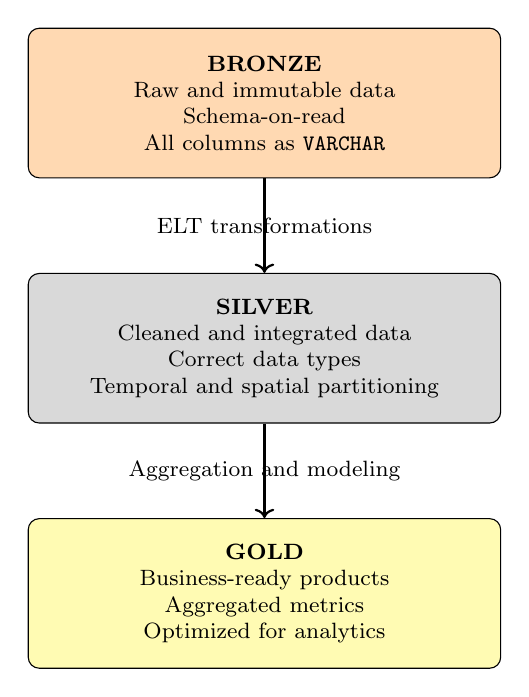
\begin{tikzpicture}[
        layer/.style={
            rectangle,
            draw,
            rounded corners,
            minimum width=6cm,
            minimum height=1.9cm,
            align=center,
            font=\footnotesize
        },
        arrow/.style={
            ->,
            thick
        }
    ]
    
    % Layers (top to bottom)
    \node[layer, fill=orange!30] (bronze) {
        \textbf{BRONZE}\\
        Raw and immutable data\\
        Schema-on-read\\
        All columns as \texttt{VARCHAR}
    };
    
    \node[layer, fill=gray!30, below=1.2cm of bronze] (silver) {
        \textbf{SILVER}\\
        Cleaned and integrated data\\
        Correct data types\\
        Temporal and spatial partitioning
    };
    
    \node[layer, fill=yellow!30, below=1.2cm of silver] (gold) {
        \textbf{GOLD}\\
        Business-ready products\\
        Aggregated metrics\\
        Optimized for analytics
    };
    
    % Arrows
    \draw[arrow] (bronze) -- node {\footnotesize ELT transformations} (silver);
    \draw[arrow] (silver) -- node {\footnotesize Aggregation and modeling} (gold);
    
    \end{tikzpicture}
    \caption{Three-tier lakehouse data pipeline.}
\end{figure}


\subsubsection*{Bronze Layer}
\begin{figure}[H]
    \centering
    \includegraphics[width=0.85\linewidth]{images/bronze_diagram.png}
    \caption{Bronze layer schema representing the raw ingestion of mobility and demographic data.}
    \label{fig:placeholder}
\end{figure}

\subsubsection*{Silver Layer}
\begin{figure}[H]
    \centering
    \includegraphics[width=\linewidth]{images/silver_diagram.png}
    \caption{Silver layer schema showing cleaned, standardized, and integrated datasets.}
    \label{fig:placeholder}
\end{figure}

\subsubsection*{Gold Layer}
\begin{figure}[H]
    \centering
    \includegraphics[width=0.7\linewidth]{images/gold_diagram.png}
    \caption{Gold layer schema illustrating business-ready analytical data products.}
    \label{fig:gold_schema}
\end{figure}

%%%%%%%%%%%%%%%%%%%%%%%%%%%%%%%%%%%%%%%%%%%%%%%%%%%%%%%%%%%%%%%%%%%%
% Lakehouse Map
%%%%%%%%%%%%%%%%%%%%%%%%%%%%%%%%%%%%%%%%%%%%%%%%%%%%%%%%%%%%%%%%%%%%
\addcontentsline{toc}{section}{Appendix B. Data sheets}
\section*{Appendix B. Data Sheets}

\subsection{Bronze Layer}

\subsubsection*{Data Sheet: \texttt{bronze\_mitma\_od\_municipios}}
\begin{itemize}
    \item \textbf{Description:} Raw origin-destination mobility matrices by municipality, date, and hour from MITMA RSS feeds.
    \item \textbf{Grain:} One row per origin zone, destination zone, date, hour, and demographic segment.
    \item \textbf{Sources:} MITMA Estudios Básicos RSS feeds
    \item \textbf{Tracking:} \texttt{source\_file} column contains URL of source CSV file
\end{itemize}

\begin{longtable}{p{3cm} p{2cm} p{1.5cm} p{1.8cm} p{6cm}}
    \caption{Technical Data Sheet for the bronze\_mitma\_od\_municipios Table} \\
    \toprule
    \textbf{Column} & \textbf{Type} & \textbf{Unit} & \textbf{Nullable} & \textbf{Description} \\
    \midrule
    fecha & TIMESTAMP & -- & No & Date (parsed from YYYYMMDD format in source CSV)\\
    periodo & VARCHAR & -- & Yes & Hour of day (0-23)\\
    origen & VARCHAR & -- & No & Origin zone identifier\\
    destino & VARCHAR & -- & No & Destination zone identifier\\
    viajes & VARCHAR & trips & No & Number of trips (as string)\\
    viajes\_km & VARCHAR & trip-km & No & Total distance traveled (as string)\\
    distancia & VARCHAR & km & Yes & Distance category or band\\
    residencia & VARCHAR & -- & Yes & Residence classification\\
    source\_file & VARCHAR & -- & No & URL of source CSV file\\
    loaded\_at & TIMESTAMP & -- & No & Timestamp of ingestion\\
    \bottomrule
\end{longtable}

\subsubsection*{Data Sheet: \texttt{bronze\_mitma\_municipios}}
\begin{itemize}
    \item \textbf{Description:} Raw zoning reference data including geometric boundaries for municipalities.
    \item \textbf{Grain:} One row per spatial zone.
    \item \textbf{Sources:} MITMA zoning shapefile exports
    \item \textbf{Tracking:} Single ingestion, no source\_file column
\end{itemize}

\begin{longtable}{p{3cm} p{2.5cm} p{1.8cm} p{7cm}}
    \caption{Technical Data Sheet for the bronze\_mitma\_municipios Table} \\
    \toprule
    \textbf{Column} & \textbf{Type} & \textbf{Nullable} & \textbf{Description}\\
    \midrule
    ID & VARCHAR & No & Unique spatial zone identifier\\
    Nombre & VARCHAR & No & Human-readable zone name\\
    geometry & VARCHAR & No & WKT (Well-Known Text) representation of polygon geometry\\
    loaded\_at & TIMESTAMP & No & Timestamp of ingestion\\
    \bottomrule
\end{longtable}

\subsubsection*{Data Sheet: \texttt{bronze\_ine\_municipios}}
\begin{itemize}
    \item \textbf{Description:} Catalog of Spanish municipalities with INE codes and names from INE API.
    \item \textbf{Grain:} One row per municipality.
    \item \textbf{Sources:} INE API (JSON format)
    \item \textbf{Tracking:} \texttt{source\_url} column contains API endpoint URL
\end{itemize}

\begin{longtable}{p{3cm} p{2.5cm} p{1.8cm} p{7cm}}
    \caption{Technical Data Sheet for the bronze\_ine\_municipios Table} \\
    \toprule
    \textbf{Column} & \textbf{Type} & \textbf{Nullable} & \textbf{Description}\\
    \midrule
    Id & VARCHAR & No & INE internal identifier\\
    Codigo & VARCHAR & No & INE municipality code\\
    Nombre & VARCHAR & No & Municipality name\\
    source\_url & VARCHAR & No & INE API endpoint URL\\
    loaded\_at & TIMESTAMP & No & Timestamp of ingestion\\
    \bottomrule
\end{longtable}

\subsubsection*{Data Sheet: \texttt{bronze\_ine\_empresas\_municipio}}
\begin{itemize}
    \item \textbf{Description:} Number of registered companies per municipality and year from INE API.
    \item \textbf{Grain:} One row per municipality and year (nested JSON structure).
    \item \textbf{Sources:} INE API (JSON format with nested Data array)
    \item \textbf{Tracking:} \texttt{source\_url} column contains API endpoint URL with year parameter
\end{itemize}

\begin{longtable}{p{3cm} p{2cm} p{1.5cm} p{1.8cm} p{6cm}}
    \caption{Technical Data Sheet for the bronze\_ine\_empresas\_municipio Table} \\
    \toprule
    \textbf{Column} & \textbf{Type} & \textbf{Unit} & \textbf{Nullable} & \textbf{Description} \\
    \midrule
    Codigo & VARCHAR & -- & No & INE municipality code\\
    Nombre & VARCHAR & -- & No & Municipality name\\
    Data & VARCHAR & -- & No & JSON array string containing year-value pairs\\
    source\_url & VARCHAR & -- & No & INE API endpoint URL\\
    loaded\_at & TIMESTAMP & -- & No & Timestamp of ingestion\\
    \bottomrule
\end{longtable}

\subsubsection*{Data Sheet: \texttt{bronze\_ine\_poblacion\_municipio}}
\begin{itemize}
    \item \textbf{Description:} Population counts by municipality, sex, and year from INE API.
    \item \textbf{Grain:} One row per municipality and year (nested JSON structure).
    \item \textbf{Sources:} INE API (JSON format with nested Data array)
    \item \textbf{Tracking:} \texttt{source\_url} column contains API endpoint URL with year parameter
\end{itemize}

\begin{longtable}{p{3cm} p{2cm} p{1.5cm} p{1.8cm} p{6cm}}
    \caption{Technical Data Sheet for the bronze\_ine\_poblacion\_municipio Table} \\
    \toprule
    \textbf{Column} & \textbf{Type} & \textbf{Unit} & \textbf{Nullable} & \textbf{Description} \\
    \midrule
    Codigo & VARCHAR & -- & No & INE municipality code\\
    Nombre & VARCHAR & -- & No & Municipality name\\
    Data & VARCHAR & -- & No & JSON array string containing year-sex-value tuples\\
    source\_url & VARCHAR & -- & No & INE API endpoint URL\\
    loaded\_at & TIMESTAMP & -- & No & Timestamp of ingestion\\
    \bottomrule
\end{longtable}

\subsubsection*{Data Sheet: \texttt{bronze\_ine\_renta\_municipio}}
\begin{itemize}
    \item \textbf{Description:} Average income per capita by municipality and year from INE API.
    \item \textbf{Grain:} One row per municipality and year (nested JSON structure).
    \item \textbf{Sources:} INE API (JSON format with nested Data array)
    \item \textbf{Tracking:} \texttt{source\_url} column contains API endpoint URL with year parameter
\end{itemize}

\begin{longtable}{p{3cm} p{2cm} p{1.5cm} p{1.8cm} p{6cm}}
    \caption{Technical Data Sheet for the bronze\_ine\_renta\_municipio Table} \\
    \toprule
    \textbf{Column} & \textbf{Type} & \textbf{Unit} & \textbf{Nullable} & \textbf{Description} \\
    \midrule
    Codigo & VARCHAR & -- & No & INE municipality code\\
    Nombre & VARCHAR & -- & No & Municipality name\\
    Data & VARCHAR & -- & No & JSON array string containing year-value pairs\\
    source\_url & VARCHAR & -- & No & INE API endpoint URL\\
    loaded\_at & TIMESTAMP & -- & No & Timestamp of ingestion\\
    \bottomrule
\end{longtable}

\subsubsection*{Data Sheet: \texttt{bronze\_mitma\_ine\_relations}}
\begin{itemize}
    \item \textbf{Description:} Mapping table connecting MITMA zone identifiers to INE municipality codes.
    \item \textbf{Grain:} One row per MITMA-INE relationship.
    \item \textbf{Sources:} MITMA CSV file from movilidad-opendata.mitma.es
    \item \textbf{Tracking:} \texttt{source\_file} column contains source CSV URL
\end{itemize}

\begin{longtable}{p{3cm} p{2.5cm} p{1.8cm} p{7cm}}
    \caption{Technical Data Sheet for the bronze\_mitma\_ine\_relations Table} \\
    \toprule
    \textbf{Column} & \textbf{Type} & \textbf{Nullable} & \textbf{Description}\\
    \midrule
    municipio\_mitma & VARCHAR & No & MITMA zone identifier\\
    municipio\_ine & VARCHAR & No & INE municipality code\\
    source\_file & VARCHAR & No & Source CSV file URL\\
    loaded\_at & TIMESTAMP & No & Timestamp of ingestion\\
    \bottomrule
\end{longtable}

\subsubsection*{Data Sheet: \texttt{bronze\_spanish\_holidays}}
\begin{itemize}
    \item \textbf{Description:} National holidays for Spain generated programmatically using Python's holidays library.
    \item \textbf{Grain:} One row per holiday date.
    \item \textbf{Sources:} Python holidays library (no external file)
    \item \textbf{Tracking:} No source tracking (programmatically generated)
\end{itemize}

\begin{longtable}{p{3cm} p{2.5cm} p{1.8cm} p{7cm}}
    \caption{Technical Data Sheet for the bronze\_spanish\_holidays Table} \\
    \toprule
    \textbf{Column} & \textbf{Type} & \textbf{Nullable} & \textbf{Description}\\
    \midrule
    date & DATE & No & Holiday date\\
    name & VARCHAR & No & Holiday name\\
    loaded\_at & TIMESTAMP & No & Timestamp of ingestion\\
    \bottomrule
\end{longtable}

\subsection{Silver Layer}

\subsubsection*{Data Sheet: \texttt{silver\_mitma\_ine\_mapping}}
\begin{itemize}
    \item \textbf{Description:} Mapping table establishing relationships between MITMA zone identifiers and INE municipality codes, with normalized names for fuzzy matching.
    \item \textbf{Grain:} One row per valid MITMA-INE relationship.
    \item \textbf{Sources:} \texttt{bronze\_ine\_municipios}, \texttt{bronze\_mitma\_ine\_relations}
\end{itemize}

\begin{longtable}{p{3cm} p{2.5cm} p{1.8cm} p{7cm}}
    \caption{Technical Data Sheet for the silver\_mitma\_ine\_mapping Table} \\
    \toprule
    \textbf{Column} & \textbf{Type} & \textbf{Nullable} & \textbf{Description}\\
    \midrule
    nombre & STRING & No & Normalized zone name (lowercase, accents removed, trimmed)\\
    codigo\_ine & VARCHAR & No & INE municipality code\\
    municipio\_mitma & VARCHAR & No & MITMA zone identifier\\
    \bottomrule
\end{longtable}

\subsubsection*{Data Sheet: \texttt{silver\_ine\_all}}
\begin{itemize}
    \item \textbf{Description:} Socioeconomic and demographic indicators derived from INE data, harmonized at the zone level.
    \item \textbf{Grain:} One row per zone and year.
    \item \textbf{Sources:} INE (Instituto Nacional de Estadística)
\end{itemize}

\begin{longtable}{p{3cm} p{2cm} p{1.5cm} p{1.8cm} p{6cm}}
    \caption{Technical Data Sheet for the silver\_ine\_all Table} \\
    \toprule
    \textbf{Column} & \textbf{Type} & \textbf{Unit} & \textbf{Nullable} & \textbf{Description} \\
    \midrule
    id & VARCHAR & -- & No & Zone identifier\\
    nombre & STRING & -- & No & Zone name\\
    empresas & DOUBLE & count & No & Number of registered companies in the zone\\
    renta\_media & DOUBLE & EUR & No & Average income per capita\\
    poblacion\_total & DOUBLE & persons & No & Total population\\
    poblacion\_hombres & DOUBLE & persons & No & Male population  \\
    poblacion\_mujeres & DOUBLE & persons & No & Female population\\
    year & INTEGER & year & No & Reference year of the indicators\\
    \bottomrule
\end{longtable}

\subsubsection*{Data Sheet: \texttt{silver\_zones}}
\begin{itemize}
    \item \textbf{Description:} Reference table defining spatial zones and their geometric properties.
    \item \textbf{Grain:} One row per spatial zone.
    \item \textbf{Sources:} MITMA zoning files, INE spatial references
\end{itemize}

\begin{longtable}{p{3cm} p{2.5cm} p{1.8cm} p{7cm}}
    \caption{Technical Data Sheet for the silver\_zones Table} \\
    \toprule
    \textbf{Column} & \textbf{Type} & \textbf{Nullable} & \textbf{Description}\\
    \midrule
    id & VARCHAR & No & Unique spatial zone identifier\\
    nombre & STRING & No & Human-readable zone name\\
    geometry\_obj & GEOMETRY & No & Polygon geometry defining zone boundaries\\
    centroid & POINT & No & Geometric centroid of the zone\\
    \bottomrule
\end{longtable}

\subsubsection*{Data Sheet: \texttt{silver\_mitma\_od}}
\begin{itemize}
    \item \textbf{Description:} Cleaned origin--destination mobility flows between spatial zones with temporal enrichment flags.
    \item \textbf{Grain:} One row per origin zone, destination zone, date, hour, and residence classification.
    \item \textbf{Sources:} \texttt{bronze\_mitma\_od\_municipios}, \texttt{bronze\_spanish\_holidays}
    \item \textbf{Partitioning:} Partitioned by \texttt{year(fecha), month(fecha), day(fecha)}
\end{itemize}

\begin{longtable}{p{3cm} p{2cm} p{1.5cm} p{1.8cm} p{6cm}}
    \caption{Technical Data Sheet for the silver\_mitma\_od Table} \\
    \toprule
    \textbf{Column} & \textbf{Type} & \textbf{Unit} & \textbf{Nullable} & \textbf{Description} \\
    \midrule
    fecha & TIMESTAMP & -- & No & Observation date and hour\\
    origen\_zone\_id & VARCHAR & -- & No & Origin zone identifier\\
    destino\_zone\_id & VARCHAR & -- & No & Destination zone identifier\\
    viajes & DOUBLE & trips & No & Total number of observed trips \\
    viajes\_km & DOUBLE & trip-km & No & Total distance traveled in trips\\
    residencia & VARCHAR & -- & No & Residence classification of travelers\\
    is\_weekend & BOOLEAN & -- & No & Flag indicating if date falls on weekend\\
    is\_holiday & BOOLEAN & -- & No & Flag indicating if date is a national holiday\\
    \bottomrule
\end{longtable}

\subsubsection*{Data Sheet: \texttt{silver\_mitma\_distances}}
\begin{itemize}
    \item \textbf{Description:} Precomputed distances between origin and destination zones.
    \item \textbf{Grain:} One row per origin--destination zone pair.
    \item \textbf{Sources:} Derived from spatial centroids in \texttt{silver\_zones}
\end{itemize}

\begin{longtable}{p{3cm} p{2cm} p{1.5cm} p{1.8cm} p{6cm}}
    \caption{Technical Data Sheet for the silver\_mitma\_distances Table} \\
    \toprule
    \textbf{Column} & \textbf{Type} & \textbf{Unit} & \textbf{Nullable} & \textbf{Description} \\
    \midrule
    origin & VARCHAR & -- & No & Origin zone identifier\\
    destination & VARCHAR & -- & No & Destination zone identifier\\
    distance\_km & DOUBLE & km & No & Euclidean distance between zone centroids\\
    \bottomrule
\end{longtable}

\subsubsection*{Data Sheet: \texttt{silver\_od\_quality}}

\begin{itemize}
    \item \textbf{Description:} Quality and diagnostic metrics computed for the \texttt{silver\_mitma\_od} table.
    \item \textbf{Grain:} One row per origin zone, destination zone, and date.
    \item \textbf{Sources:} Derived from \texttt{silver\_mitma\_od} and population data
\end{itemize}

\begin{longtable}{p{5cm} p{2cm} p{1.5cm} p{1.8cm} p{4cm}}
    \caption{Technical Data Sheet for the silver\_od\_quality Table} \\
    \toprule
    \textbf{Column} & \textbf{Type} & \textbf{Unit} & \textbf{Nullable} & \textbf{Description}\\
    \midrule
    origen\_zone\_id & VARCHAR & -- & No & Origin zone identifier\\
    destino\_zone\_id & VARCHAR & -- & No & Destination zone identifier\\
    fecha & DATETIME & -- & No & Observation date\\
    viajes\_per\_capita & DOUBLE & trips & No & Trips normalized by origin population\\
    km\_per\_capita & DOUBLE & km & No & Distance traveled normalized by population\\
    flag\_negative\_viajes & BOOLEAN & -- & No & Flag indicating negative trip counts\\
    flag\_negative\_viajes\_km & BOOLEAN & -- & No & Flag indicating negative distance values\\
    z\_viajes\_per\_capita & FLOAT & z-score & No & Standardized trips per capita metric\\
    flag\_outlier\_viajes\_per\_capita & BOOLEAN & -- & No & Outlier flag based on z-score threshold\\
    \bottomrule
\end{longtable}

\subsection{Gold Layer}

\subsubsection*{Data Sheet: \texttt{gold\_typical\_day\_od\_hourly}}
\begin{itemize}
    \item \textbf{Description:} Average hourly mobility profile. Aggregates silver layer flows to obtain an analytical ``typical day'', allowing observation of peak and off-peak patterns.
    \item \textbf{Grain:} One row per origin zone, destination zone, date, and hour.
    \item \textbf{Sources:} \texttt{silver\_od}
\end{itemize}

\begin{longtable}{p{3cm} p{2cm} p{1.5cm} p{1.8cm} p{6cm}}
    \caption{Technical Data Sheet for the gold\_typical\_day\_od\_hourly Table} \\
    \toprule
    \textbf{Column} & \textbf{Type} & \textbf{Unit} & \textbf{Nullable} & \textbf{Description} \\
    \midrule
    origin\_id & VARCHAR & -- & No & Unique identifier of the zone where the trip begins.\\
    destination\_id & VARCHAR & -- & No & Unique identifier of the zone where the trip ends.\\
    date & DATE & -- & No & Specific date of the observation for time-series analysis.\\
    hour & INTEGER & hour & No & Hour of the day (0-23) when the trips occurred.\\
    avg\_trips & DOUBLE & trips & No & Average number of trips recorded for that specific hour and date.\\
    avg\_km & DOUBLE & km & No & Average total distance traveled for trips in that specific time window.\\
    \bottomrule
\end{longtable}

\subsubsection*{Data Sheet: \texttt{gold\_gravity\_mismatch}}
\begin{itemize}
    \item \textbf{Description:} Comparison between observed actual mobility and theoretical mobility predicted by a Gravity Model based on mass (population and companies) and distance.
    \item \textbf{Grain:} One row per origin zone, destination zone, and date.
    \item \textbf{Sources:} \texttt{silver\_mitma\_od}, \texttt{silver\_ine\_all}, \texttt{silver\_mitma\_distances}
\end{itemize}

\begin{longtable}{p{3cm} p{2cm} p{1.5cm} p{1.8cm} p{6cm}}
    \caption{Technical Data Sheet for the gold\_gravity\_mismatch Table} \\
    \toprule
    \textbf{Column} & \textbf{Type} & \textbf{Unit} & \textbf{Nullable} & \textbf{Description} \\
    \midrule
    origin\_id & VARCHAR & -- & No & Identifier for the origin zone.\\
    destination\_id & VARCHAR & -- & No & Identifier for the destination zone.\\
    date & DATE & -- & No & Date of the travel observation.\\
    actual\_trips & DOUBLE & trips & No & Real number of trips observed in the mobility data.\\
    estimated\_trips & DOUBLE & trips & No & Theoretical trips predicted by the model based on population, companies and distance.\\
    mismatch\_ratio & DOUBLE & ratio & Yes & Ratio of actual trips to estimated trips.\\
    \bottomrule
\end{longtable}

\subsubsection*{Data Sheet: \texttt{gold\_zone\_functional\_type}}
\begin{itemize}
    \item \textbf{Description:} Classification of zones based on their predominant mobility behavior, calculated using K-Means clustering on inbound and outbound flows.
    \item \textbf{Grain:} One row per spatial zone.
    \item \textbf{Sources:} \texttt{silver\_mitma\_od}, \texttt{silver\_zones}, Scikit-learn Clustering
\end{itemize}

\begin{longtable}{p{3cm} p{2.5cm} p{1.8cm} p{7cm}}
    \caption{Technical Data Sheet for the gold\_zone\_functional\_type Table} \\
    \toprule
    \textbf{Column} & \textbf{Type} & \textbf{Nullable} & \textbf{Description}\\
    \midrule
    zone\_id & VARCHAR & No & Unique identifier of the spatial zone.\\
    functional\_type & STRING & No & Label from the model: `Residential' (high morning outbound flows) or `Non-residential' (labor/commercial activity centers).\\
    \bottomrule
\end{longtable}

%%%%%%%%%%%%%%%%%%%%%%%%%%%%%%%%%%%%%%%%%%%%%%%%%%%%%%%%%%%%%%%%%%%%
% FIN DOCUMENTO
%%%%%%%%%%%%%%%%%%%%%%%%%%%%%%%%%%%%%%%%%%%%%%%%%%%%%%%%%%%%%%%%%%%%
\end{document}
